\section{Lezione 2016-10-24}
\subsection{TODO}
% Insert what you need. Any row is associated with the improvment or mistake
% arise. In the first column you can insert what you should resolve or change,
% instead in the second column you may put the section where to apply some
% modification.
\begin{table}[H]
\begin{center}
\begin{tabular}{|p{\textwidth}|c|}
\hline
\multicolumn{1}{|c|}{\textbf{Miglioramento}} & \textbf{Sezione} \\ \hline
Rappresentare l'associativit\`a & \ref{sec:common_subexpression} \\ \hline
Capire quale migliora porta la rinomina delle variabili morte &
\ref{sec:renaming_temporary_variable} \\ \hline
Capire quale miglioria porta lo scambio delle istruzioni &
\ref{sec:interchange_statements} \\ \hline
\end{tabular}
\end{center}
\caption{Tabella miglioramenti}
\label{tab:tab_todo}
\end{table}

\subsection{Sul generatore di codice}
Il codice prodotto dal compilatore deve essere corretto, ovvero, deve
preservare la semantica (\textit{semantic preserving}) e dovrebbe essere di
alta qualit\'a. Ci\`o implica un uso efficacie delle risorse della macchina
obiettivo ed, attraverso una serie di euristiche, produrre un buon codice
vicono a quello ottimale (la produzione di codice ottimale \`e
\textbf{indicibile}).

\begin{figure}[H]
  \centering
  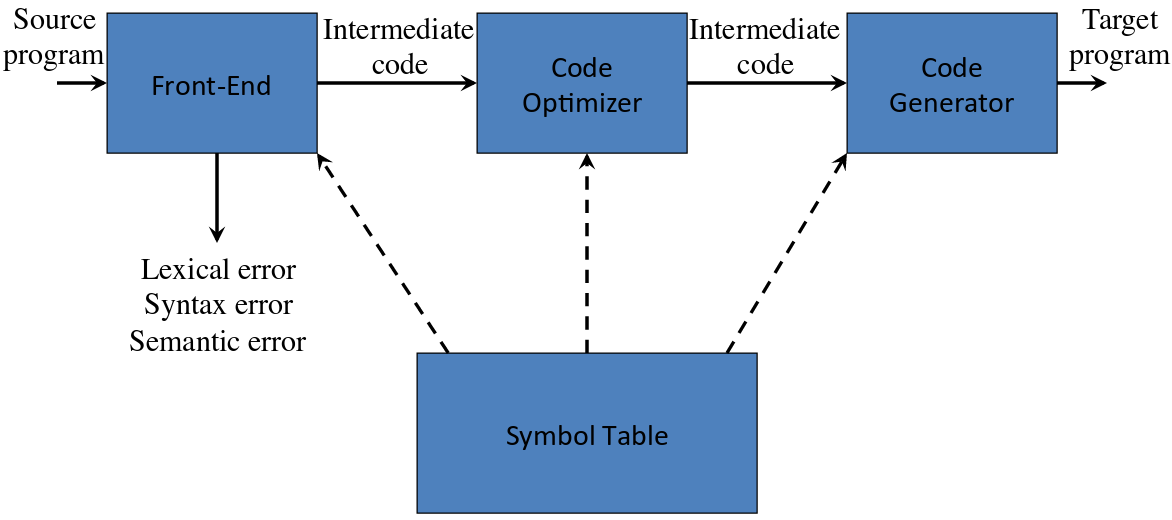
\includegraphics[scale=0.4]{res/image/code_generator_position}
  \caption{Posizione del generatori di codice}
  \label{img:code_generator_position}
\end{figure}

\subsection{Compiti del generatore}
Il \textit{code generator} ha tre compiti primari:
\begin{itemize}
\item selezione dell'istruzione
\item assegnazione ed allocazione dei registri
\item ordinamento delle istruzioni
\end{itemize}

Inoltre il compilatore pu\`o includere una fase di ottimizzazione (mappa l'IR
in input con IR ottimizzato) prima della generazione del codice.

\subsection{Variabili del generatore}
\subsubsection{L'input}
L'input del generatore \`e l'IR del codice sorgente, con i puntatori alle
informazioni salvate nella tabella dei simboli.
\subsubsection{Codice target}
Il \textit{backend} di un generatore di codice pu\`o generare differenze forme
di codice a seconda dei requisiti:
\begin{itemize}
\item codice macchina assoluto (codice eseguibile)
\item codice macchina riallocabile (file oggetto per il \textbf{linker})
\item linguaggio assembly (facilita il debuggin, ma richiede un assembly step)
\end{itemize}

\subsubsection{Architettura della macchina}
Definisce il set d'istruzioni avviabili, incluso il modello d'indirizzamento:
alto impatto sul codice generato.

Le macchine si vanno a dividire in due principali categorie:
\paragraph{CISC}
\begin{itemize}
\item istruzioni multi-clock
\item metodo d'indirizzamento complesso
\item serie di classi di registri
\item lunghezza variabile delle istruzioni in memoria
\end{itemize}
\paragraph{RISC}
\begin{itemize}
\item istruzioni single-clcok
\item molti registri
\item istruzioni a tre indirizzi
\item metodo d'indirizzamento semplice
\end{itemize}
\paragraph{Stack-based}
gli operandi sono inseriti nello stack e le operazioni sono eseguite nel top
(trattenute nei registri). In generale meno efficiente.

\subsection{Selezione dell'istruzione}
Uno comando pu\`o essere tradotto in vari modi. La scelta su quale set di
istruzioni convertirlo dipende da:
\begin{enumerate}
\item livello dell'IR
\item set d'istruzioni dell'architettura
\item la qualit\`a desiderata (es. efficienza) del codice generato
\end{enumerate}

\begin{figure}[H]
  \centering
  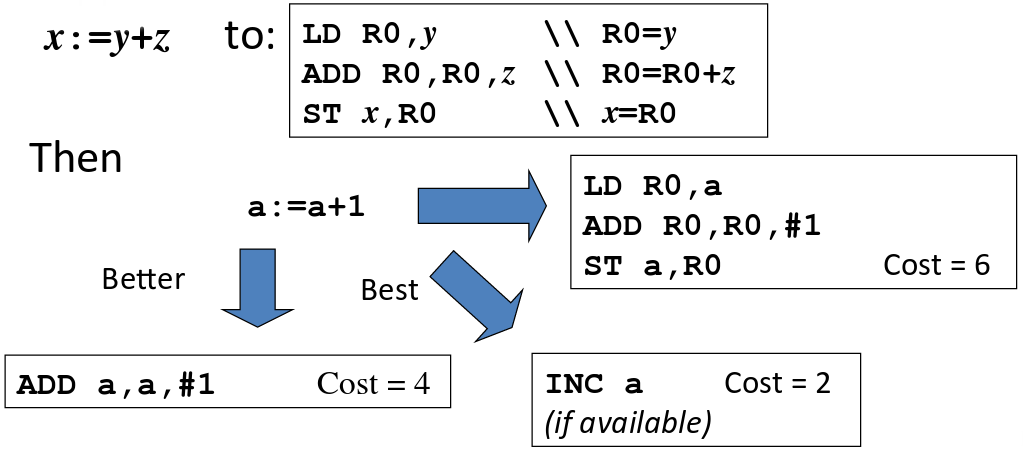
\includegraphics[scale=0.35]{res/image/choice_cost}
  \caption{Scelta del set di comandi in base al costo}
  \label{img:choice_cost}
\end{figure}

Per semplicit\`a dell'architettura possiamo definire il costo come
\begin{align*}
cost(\mathbf{OP \ dst}, \mathbf{src1}, \mathbf{src2})
&= 1 \\
&+ cost(dst\text{-}mode) \\
&+ cost(src1\text{-}mode) \\
&+ cost(src2\text{-}mode)
\end{align*}

La mappatura semplice delle singole istruzioni non garantisce una buona
qualit\`a del codice, in quanto non si va ad osservarlo nella usa interezza.

\begin{figure}[H]
  \centering
  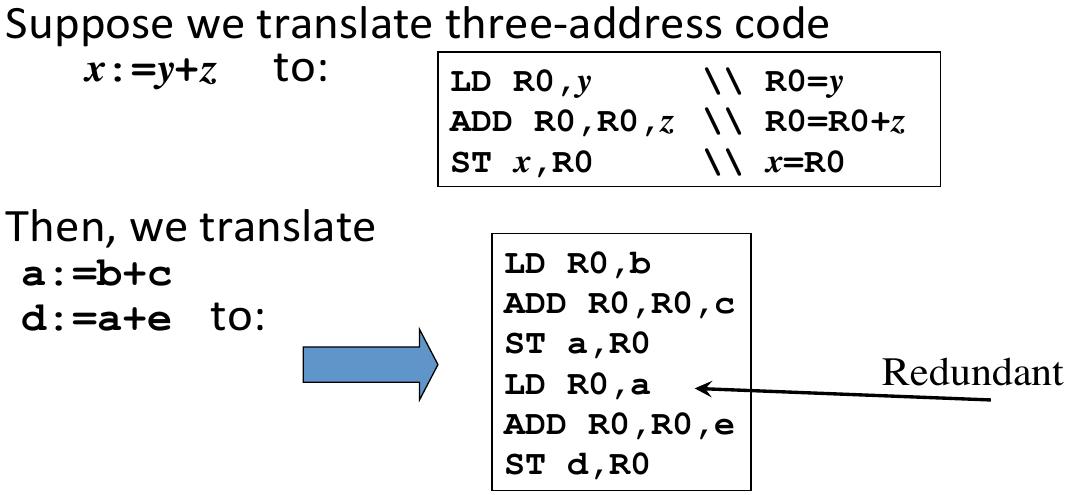
\includegraphics[scale=0.35]{res/image/needed_global_optimization}
  \caption{Necessarie ottimizzazione globali per eliminare ridondanze}
  \label{img:needed_global_optimization}
\end{figure}

Si possono fare due accorgimenti per garantire una buona qualit\`a del codice:
\paragraph{Allocazione ed assegnazione dei registri}
L'uso efficiente di un piccolo insieme di registri \`e importante per generare
buon codice. I registri sono assegnati per:
\begin{itemize}
\item \textit{Register Allocation} - per selezionare l'insieme delle variabili
che risiederanno nei registri a quel punto del codice
\item \textit{Register Assignment} - per scegliere in quale registro la
variabile risieder\'a
\end{itemize}
Trovare un insieme di registri ottimali \`e un problema in
\textit{NP-completo}.
\paragraph{Scelta dell'ordine di istruzioni}
L'ordine delle istruzioni potrebbe portare ad un miglioramento delle
prestazioni del programma. Se le istruzioni sono indipendenti, l'ordine di
valutazione pu\'o cambiare.

\begin{figure}[H]
  \centering
  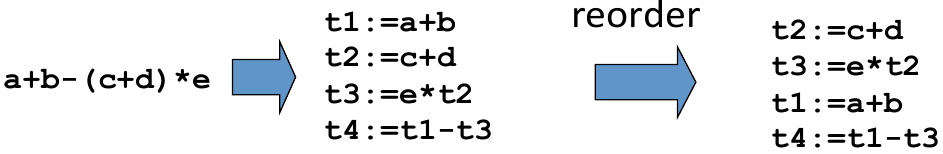
\includegraphics[scale=0.5]{res/image/reorder_variable}
  \caption{Riordinamento di variabili indipendenti}
  \label{img:reorder_variable}
\end{figure}

\subsection{Towards Flow Graphs}
Un modo per migliorare l'ordinamento, la selezione e l'allocazione dei registri
ed infine la scelta nel set d'istruzione. Noi possiamo strutturare il
three-address code come un \textit{flow graph}.

Il vantaggio del grafo \`e la miglior rappresentazione delle dipendenze lungo
le istruzioni dell'IR. Infatti alcune tecniche d'ottimizzazione sono fatte in
base alle dipendenze.

\begin{definition}[Flow Graph]
Un grafico di flusso \`e una rappresentazione a grafico di una sequenza
d'istruzioni con i spigoli che rappresentano il controllo di flusso.
\end{definition}

\textbf{I nodi} rappresentano i \textit{basic block}, la sequenza d'istruzioni
che vengono sempre eseguite insieme.

\textbf{Gli archi} \`e l'ordine d'esecuzioni dipendenti.

\subsubsection{Basic Blocks}
\begin{definition}[Basic Block]
Un blocco base \`e una sequenza d'istruzioni tale che:
\begin{itemize}
\item il controllo entra tramite solo la prima istruzione
\item il controllo lascia il blocco senza \textit{branching}, eccetto l'ultima
istruzione
\end{itemize}
\end{definition}

\begin{figure}[H]
  \centering
  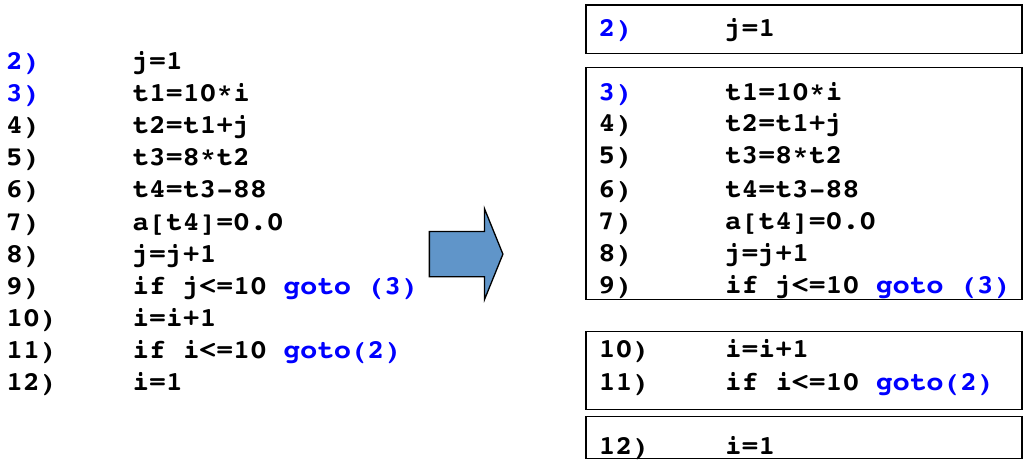
\includegraphics[scale=0.5]{res/image/basic_block}
  \caption{Blocchi base}
  \label{img:basic_block}
\end{figure}

\subsubsection{Control Flow Graph}
\begin{definition}[Control Flow Graph]
Un control flow graph \`e un grafo diretto con blocchi base $B_i$ come vertici
e come spigoli $B_i \to B_j$ sse $B_j$ pu\'o essere eseguito immediatamente
dopo $B_i$.
\end{definition}

Si definisce $B_i$ come il predecessore di $B_j$, e $B_j$ il successore di
$B_i$.

\begin{figure}[H]
  \centering
  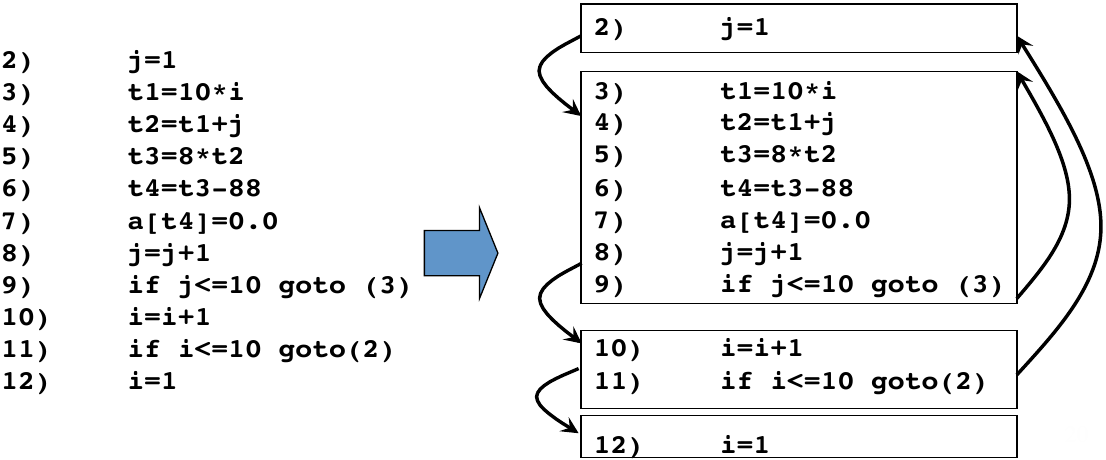
\includegraphics[scale=0.35]{res/image/control_flow_graph}
  \caption{Control Flow Graph}
  \label{img:control_flow_graph}
\end{figure}

\subsubsection{Algoritmo di partizionamento per blocchi base}
\paragraph{Input}
Una sequenza di three-address code
\paragraph{Output}
Una lista di blocchi base con ogni three-address statement in esattamente un
blocco.

\begin{enumerate}
\item Determinare l'insieme di \textit{leaders}, le prime istruzioni nei
blocchi base
\begin{itemize}
\item Il primo statement \`e il \textit{leader}
\item Ogni istruzione che \`e il target di un'istruzione $goto$ \`e un
\textit{leader}
\item Ogni istruzione che immediatamente segue un $goto$ \`e un \textit{leader}
\end{itemize}
\item Per ogni \textit{leader}, il suo blocco base consiste nel \textit{leader}
e tutte le istruzioni successive ma non includendo il prossimo \textit{leader}
o la fine del programma
\end{enumerate}

\begin{figure}[H]
  \centering
  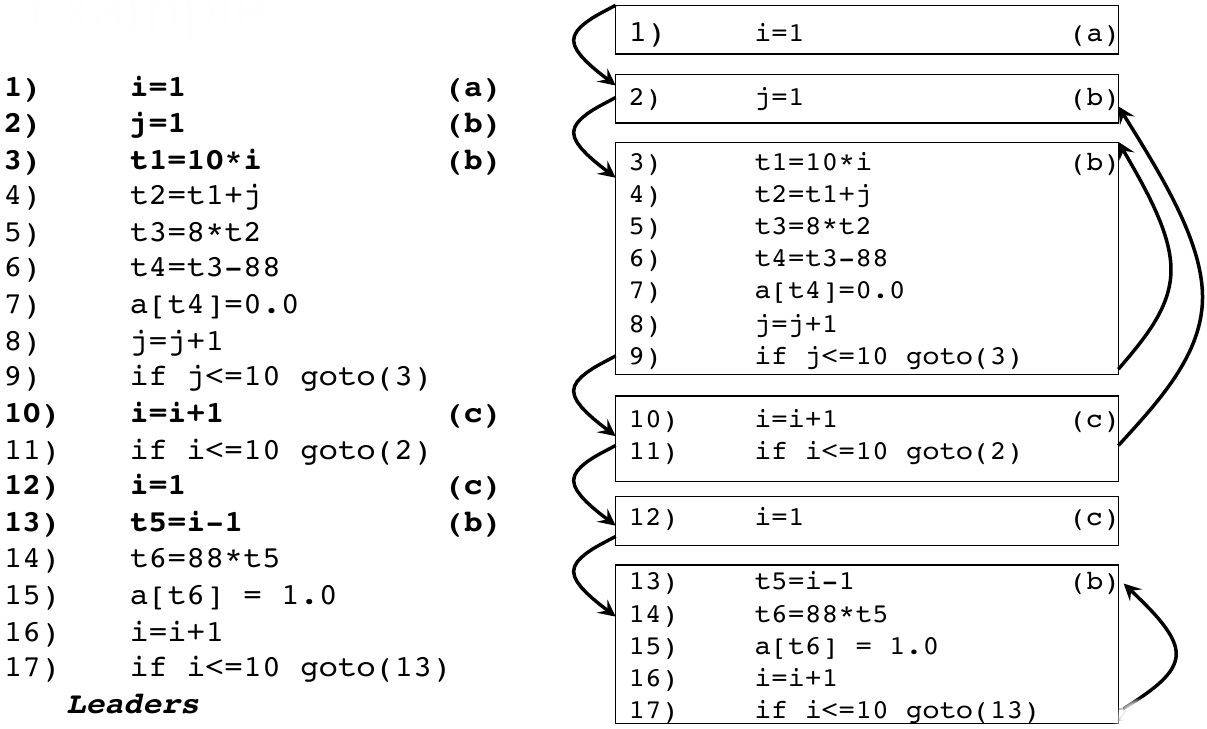
\includegraphics[scale=0.35]{res/image/leader_block}
  \caption{CFG con segnati i \textit{leader}}
  \label{img:leader_block}
\end{figure}

\subsubsection{Loop}
I programma spendono molto tempo all'interno dei loop, perci\'o identificarli e
ottimizzarli danno una buona qualit\'a del codice.

\begin{definition}[Loop]
Un loop \`e una collezione di blocchi, tale che:
\begin{itemize}
\item Tutti i blocchi nella collezione sono \textbf{fortemente connessi}
\item La collezione ha un'unica entrata, e l'unico modo per raggiungere il loop
\`e tramite lei
\end{itemize}
\end{definition}

\begin{figure}[H]
  \centering
  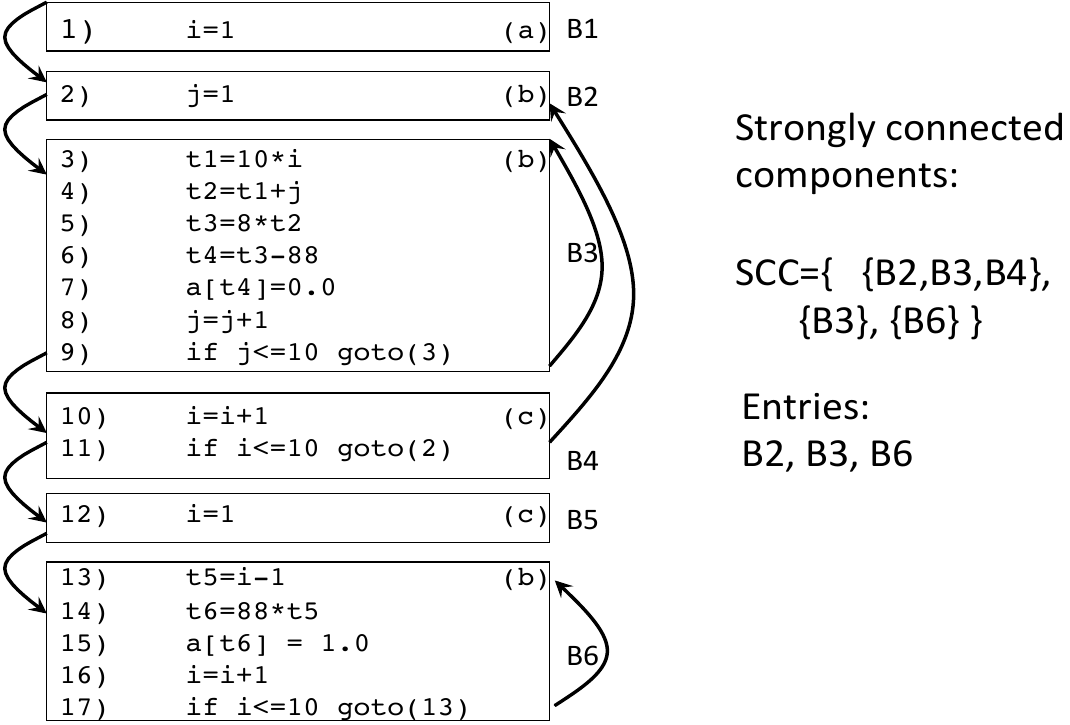
\includegraphics[scale=0.4]{res/image/loop}
  \caption{Loop}
  \label{img:loop}
\end{figure}

\subsection{Ottimizzazione locale contro globale}
\begin{definition}[Local optimization]
Tecniche di ottimizzazione del codice che lavorano sullo scope dei blocchi base
si chiamano local optimization.
\end{definition}
\begin{definition}[Global optimization]
Tecniche di ottimizzazione del codice che hanno bisogno di analizzare l'intero
CFG di un programma sono chiamate global optimization.
\end{definition}

\subsubsection{Equivalenza dei blocchi}
L'ottimizzazione locale deve assicurare che blocchi ottimizzati siano
equivalenti agli originali:

\begin{definition}[Equivalente Basic Block]
Due blocchi base si dicono equivalenti (semanticamente) se entrambi computano
lo stesso insieme d'espressioni.
\end{definition}

\begin{figure}[H]
  \centering
  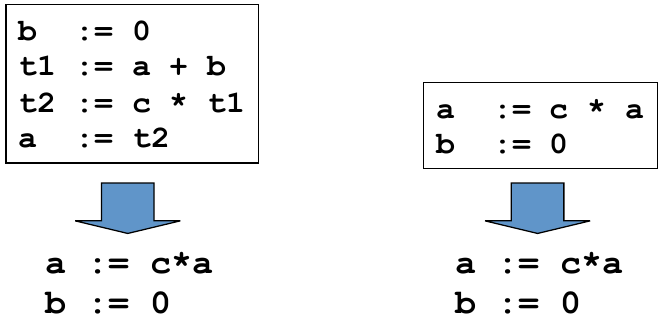
\includegraphics[scale=0.4]{res/image/equivalent_block}
  \caption{Blocchi equivalenti}
  \label{img:equivalent_block}
\end{figure}

\subsection{Ottimizzazioni basate sui DAG}
Alcune ottimizzazioni locali si mettono in luce su una rappresentazione
aciclica direzionata delle istruzioni nel blocco base. Questi DAG sono
costruiti come segue:
\begin{enumerate}
\item c'\`e un nodo nel DAG per ogni valore in input apparso nel blocco base
\item c'\`e un nodo assiociato ad ogni istruzione del blocco base
\item se l'istrusione $S$ utilizza variabili dichiarate in $S_1,...,S_n$,
allora abbiamo uno spigolo da ogni $S_i$ a $S$
\item se una variabile \`e definita nel blocco base, ma non viene utilizzata
intermanete, allora si marca come un \textit{output value}
\end{enumerate}

\begin{figure}[H]
  \centering
  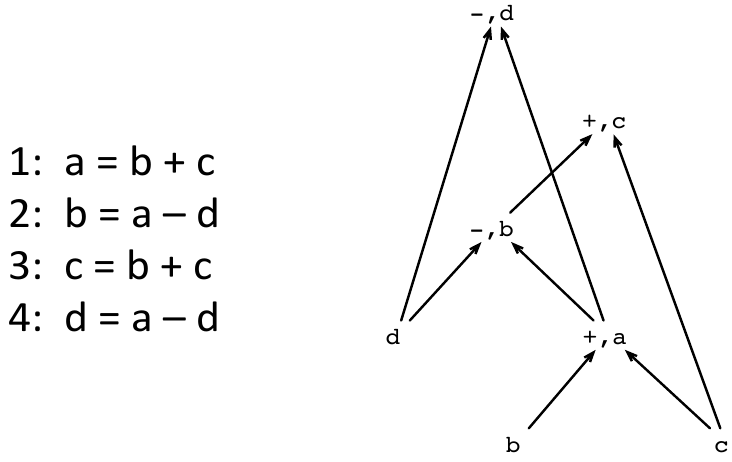
\includegraphics[scale=0.4]{res/image/dag_block}
  \caption{Rappresentazione di un blocco base mediante DAG}
  \label{img:dag_block}
\end{figure}

Nella fig.\ref{img:dag_block} abbiamo che \textbf{b,c,d} sono \textit{input
value} perch\`e vengono usati prima della loro dichiarazione, mentre le
definizioni di \textbf{c,d} sono \textit{output value} in quando non vengono
utilizzate nel blocco base.

\subsubsection{Trovare la comune sottoespressione locale}
\label{sec:common_subexpression}
L'algoritmo per la generazione del DAG pu\'o essere migliorato per identificare
espressioni gi\'a create e riutilizzarle nel caso venissero usate pi\'u volte.
Semplicemente nella creazione del nodo di un'istruzione (punto 3 dell'algoritmo
di costruzione) si va a controllare che non sia gi\'a stato creato, ed in caso
positivo il nodo diventa un \textbf{alias} dell'istruzione da inserire.

Per definire se un nodo \`e gi\'a presente nel nostro DAG si va a costruire una
tabella di hashing il cui valore \`e il nodo stesso e come chiave la segnatura:
$$(lb,v_1,...,v_n)$$
dove $lb$ \`e l'etichetta ed ogni $v_i$, con $1 <= i <= n$, \`e un figlio. Il
valore prodotto dalla funzione di hash \`e chiamato \textit{value-number}.

Perci\`o nell'inserimento di un nuovo nodo prima si fa una ricerca nella
tabella di hashing e se \`e gi\'a presente si ritorna un suo riferimento.

\begin{figure}[H]
  \centering
  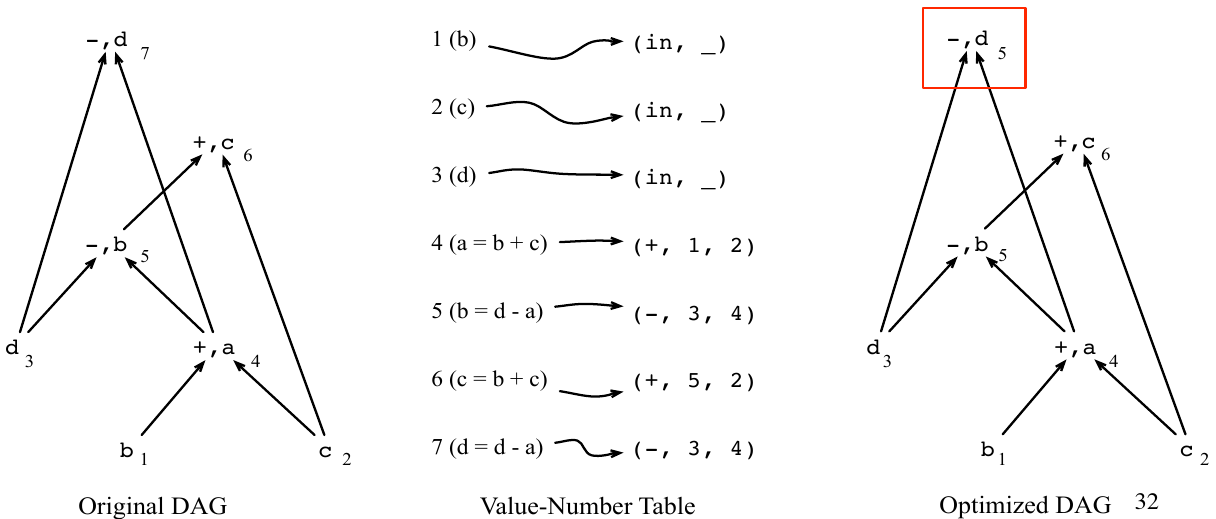
\includegraphics[scale=0.4]{res/image/original_optimized_dag}
  \caption{Uso tabella di hashing per ottimizzare il DAG}
  \label{img:original_optimized_dag}
\end{figure}

Da notare che il nodo $(+,c_{\ 6})$ non ha subito modifiche nonostante la sua
espressione, (6), coincida con l'espressione (4). Il motivo \`e per via dei
figli non coincidenti essendo che $b$ \`e stato modificato al passo (5).

I \textit{value-number} ci permettono di riferici ai nodi del nostro DAG per
la loro \textbf{semantica}, invece della rappresentazione testuale.

Olte a questa possiamo usare altre accorgimenti per trovare la sottoespressione
comune nel DAG:
\begin{itemize}
\item \textbf{commutativit\`a} - il valore di $x+y$ e $y+x$ dovrebbe essere lo
stesso
\item \textbf{identit\`a} - la comparazione $x<y$ pu\`o spesso essere
implementata come $t=x-y; \ t<0$
\item \textbf{associativit\`a} -
\end{itemize}

\subsubsection{Eliminazione del \textit{dead code}}
\`E possibile rimuovere un nodo se:
\begin{itemize}
\item il nodo \textbf{non ha discendenti} (es. \`e il nodo radice)
\item il nodo \textbf{non \`e marcato} come un \textit{output node}
\end{itemize}

Questo pattern d'eliminazione pu\`o essere iterato finch\'e non ci siano pi\`u
nodi che possono essere rimossi.

\begin{figure}[H]
  \centering
  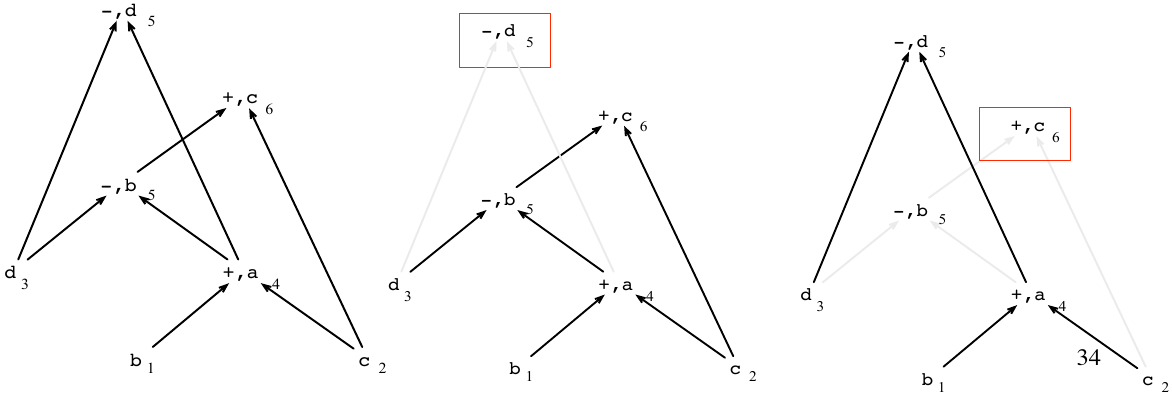
\includegraphics[scale=0.4]{res/image/remove_dead_code}
  \caption{
    Esempio rimozione $(-,d)$ o $(+,c)$ se non fossero \textit{output node}
  }
  \label{img:remove_dead_code}
\end{figure}

\subsubsection{Identit\`a algebriche}
Possiamo ridurre le identit\`a algebriche per ottimizzare il DAG. Sono mostrati
in tre modi:
\begin{itemize}
\item Identit\`a aritmetiche:
$$x+0=0+x=x; \ x*1=1*x=x; \ x-0=x; \ x/1=x;$$
\item Riduzioni in \textit{stength}:
$$x^2=x*x; \ 2*x=x+x; \ x/2=x*0.5; \ 4*x=x<<2;$$
\item Constant folding:
valutare le espressioni a \textit{compile time}, rimpiazzando il le espressioni
con il suo valore
\end{itemize}

In particolare la \textit{reduction in strength} rimpiazza alcune sequenze di
istruzioni con altre che possono essere computate in modo pi\`u efficiente.

\subsection{Ottimizzazioni Peephole}
Le \textit{peephole optimization} sono una categoria di ottimizzazioni
\textbf{locali}. Il principio \`e semplice: l'ottimizzatore analizza la
sequenza d'istruzioni all'interno di una \textbf{finestra} di piccole
dimensioni, il quale scorre sopra il codice del programma. Una volta dei
\textit{pattern} sono scoperti le ottimizzazioni sono applicate.

A seconda dei pattern individuati si vanno ad applicare varie trasformazioni.

\subsubsection{Load e store ridonanti}
Alcuni accessi in memoria sono chiaramente ridondanti:
\begin{figure}[H]
  \centering
  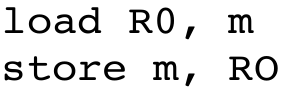
\includegraphics[scale=0.4]{res/image/redundant_load_store}
  \caption{Codice di caricamento e salvataggio ridondante}
  \label{img:redundant_load_store}
\end{figure}

Con l'utilizzo del \textit{peephole optimization} sono facilmente
rimovibili.

\subsubsection{Branch transformation}
Alcuni branch possono essere scritti mediante codice pi\`u veloce:
\begin{figure}[H]
  \centering
  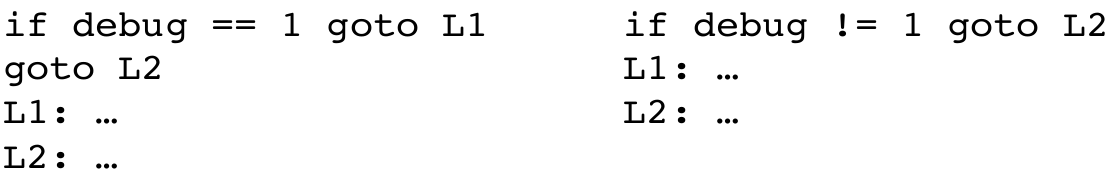
\includegraphics[scale=0.4]{res/image/branch_transformation}
  \caption{Branch equivalente ma con meno istruzioni}
  \label{img:branch_transformation}
\end{figure}

Le ottimizzazioni sono applicate oltre i limiti dei blocchi basi ma sempre su
finestre molto ridotte.

\subsubsection{Salti di salti}
Il caso da analizzare \`e quando un salto va a cadere in un'istruzione di
un'altro salto.

\begin{figure}[H]
  \centering
  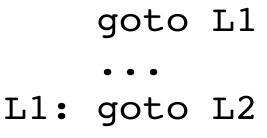
\includegraphics[scale=0.4]{res/image/jump_jump}
  \caption{Caso di un salto che salta in un'istruzione di salto}
  \label{img:jump_jump}
\end{figure}

La prima istruzione (\textit{goto L1}) potr\`a essere tranquillamente
convertita in \textit{goto L2} in quanto equivalente e risparmia l'esecuzione
di un'istruzione di salto.

Invece non \`e possibile portare modifiche al secondo \textit{jump} con
leggerezza. In caso di modifica, un'ottimizzazione di \textit{peephole} sarebbe
quella di eliminarlo, cosi riducendo lo spazio del programma. Tuttavia per
eseguire una tale operazione bisogna sapere se vi sono altre istruzioni di
\textit{jump} che puntato proprio ad $L1$. Se non vi fossero altri salti
nel programma allora si potrebbe tranquillamente \textbf{elinimarlo}.
\begin{figure}[H]
  \centering
  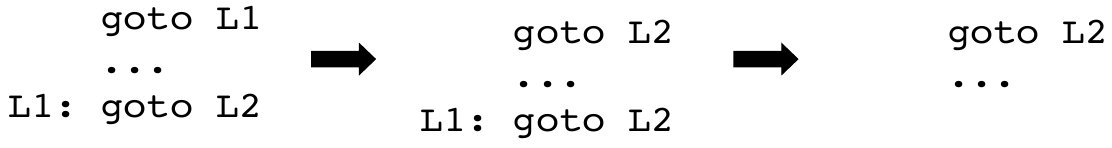
\includegraphics[scale=0.4]{res/image/remove_jump_jump}
  \caption{Ottimizzazione peephole completa sui salti di salti}
  \label{img:remove_jump_jump}
\end{figure}

In altri casi non potrebbe essere possibile applicare l'eliminazione del
secondo \textit{jump} ma solo la modifica dell'etichetta obiettivo del primo.
\begin{figure}[H]
  \centering
  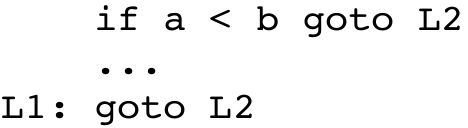
\includegraphics[scale=0.4]{res/image/no_remove_jump_jump}
  \caption{Ottimizzazione peephole solo sull'etichetta target}
  \label{img:no_remove_jump_jump}
\end{figure}

\subsubsection{Rinomina variabili temporanee}
\label{sec:renaming_temporary_variable}
Variabili temporanee che sono morte alla fine del blocco possono essere
rinominate in modo sicuro.
\begin{figure}[H]
  \centering
  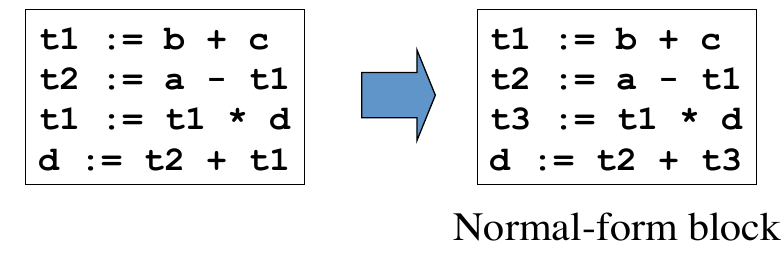
\includegraphics[scale=0.4]{res/image/renaming_variable}
  \caption{Rinomina variabili temporanee morte}
  \label{img:renaming_variable}
\end{figure}

\subsubsection{Scambio delle istruzioni}
\label{sec:interchange_statements}
Istruzioni indipendenti possono essere riordinate.
\begin{figure}[H]
  \centering
  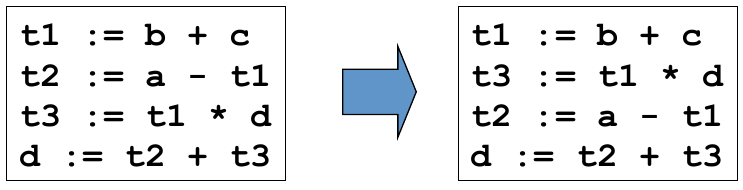
\includegraphics[scale=0.4]{res/image/interchange_statement}
  \caption{Riordinamento delle istruzioni}
  \label{img:interchange_statement}
\end{figure}

Da notare che la forma normale dei blocchi base permette lo scambio delle
istruzioni in tutti i modi possibili.
